\documentclass{beamer}
\usepackage{xeCJK}
\usepackage[bit,zh]{collegeBeamer}

\definecolor{hrefcol}{RGB}{0, 0, 255} % Example: blue color

% meta-data
\title{基于不同模型的卫生资源预测与配置}
\subtitle{文献阅读报告}
\author{{黄宇辰}}
\date{2025.8.26}

% document body
\begin{document}

    \maketitle

    \begin{frame}
        \begin{abstract}
            \qquad 通过在文件搜索网站查询, 发现不同的数学模型在卫生资源预测与配置中有非常广泛的应用, 包括\textbf{灰色-回归组合模型}, 以及\textbf{DEA-Malmquist指数模型}等数学模型. 

            \qquad 通过比较两篇论文\textbf{基于灰色－回归组合模型的淄博市卫生资源预测}与\textbf{基于DEA-Malmquist分析的广东省城市公立医院资源配置效率研究}的结果, 可以看出这两种模型各有优劣, 但都为卫生资源的合理配置提供了重要的参考依据.
        \end{abstract}
    \end{frame}

    \section{论文选取}

    \begin{frame}{选取过程}{\thesection \, \secname}
        \qquad 首先依托中国知网(CNKI)与Web of Science(WoS)两大权威学术数据库开展检索. 以\textbf{卫生资源预测}、\textbf{卫生资源配置}、\textbf{数学模型}、\textbf{2025年} 为核心检索词, 精准锁定论文的研究范围. 

        \qquad 经标题、摘要精读, 剔除以下内容: 模型应用与卫生资源无关(如工业资源配置、农业资源模型); 仅提及资源分配概念以及数学模型理论, 无具体构建与求解过程; 重复发表或内容不完整的论文. 

        \qquad 最终筛选出 \textbf{2篇核心论文}, 覆盖不同数学模型类型, 满足作业对比分析需求. 
    \end{frame}

    \begin{frame}{选取结果}{\thesection \, \secname}
       \begin{columns}
            \begin{column}{0.45\textwidth}
               \qquad 最终选择了两篇核心论文:
               \begin{itemize}
                   \item \textbf{基于灰色－回归组合模型的淄博市卫生资源预测}
                   \item \textbf{基于DEA-Malmquist分析的广东省城市公立医院资源配置效率研究}
               \end{itemize}
            \end{column}
            \begin{column}{0.55\textwidth}
                
\includegraphics[width=0.8\textwidth]{essay1.png}
                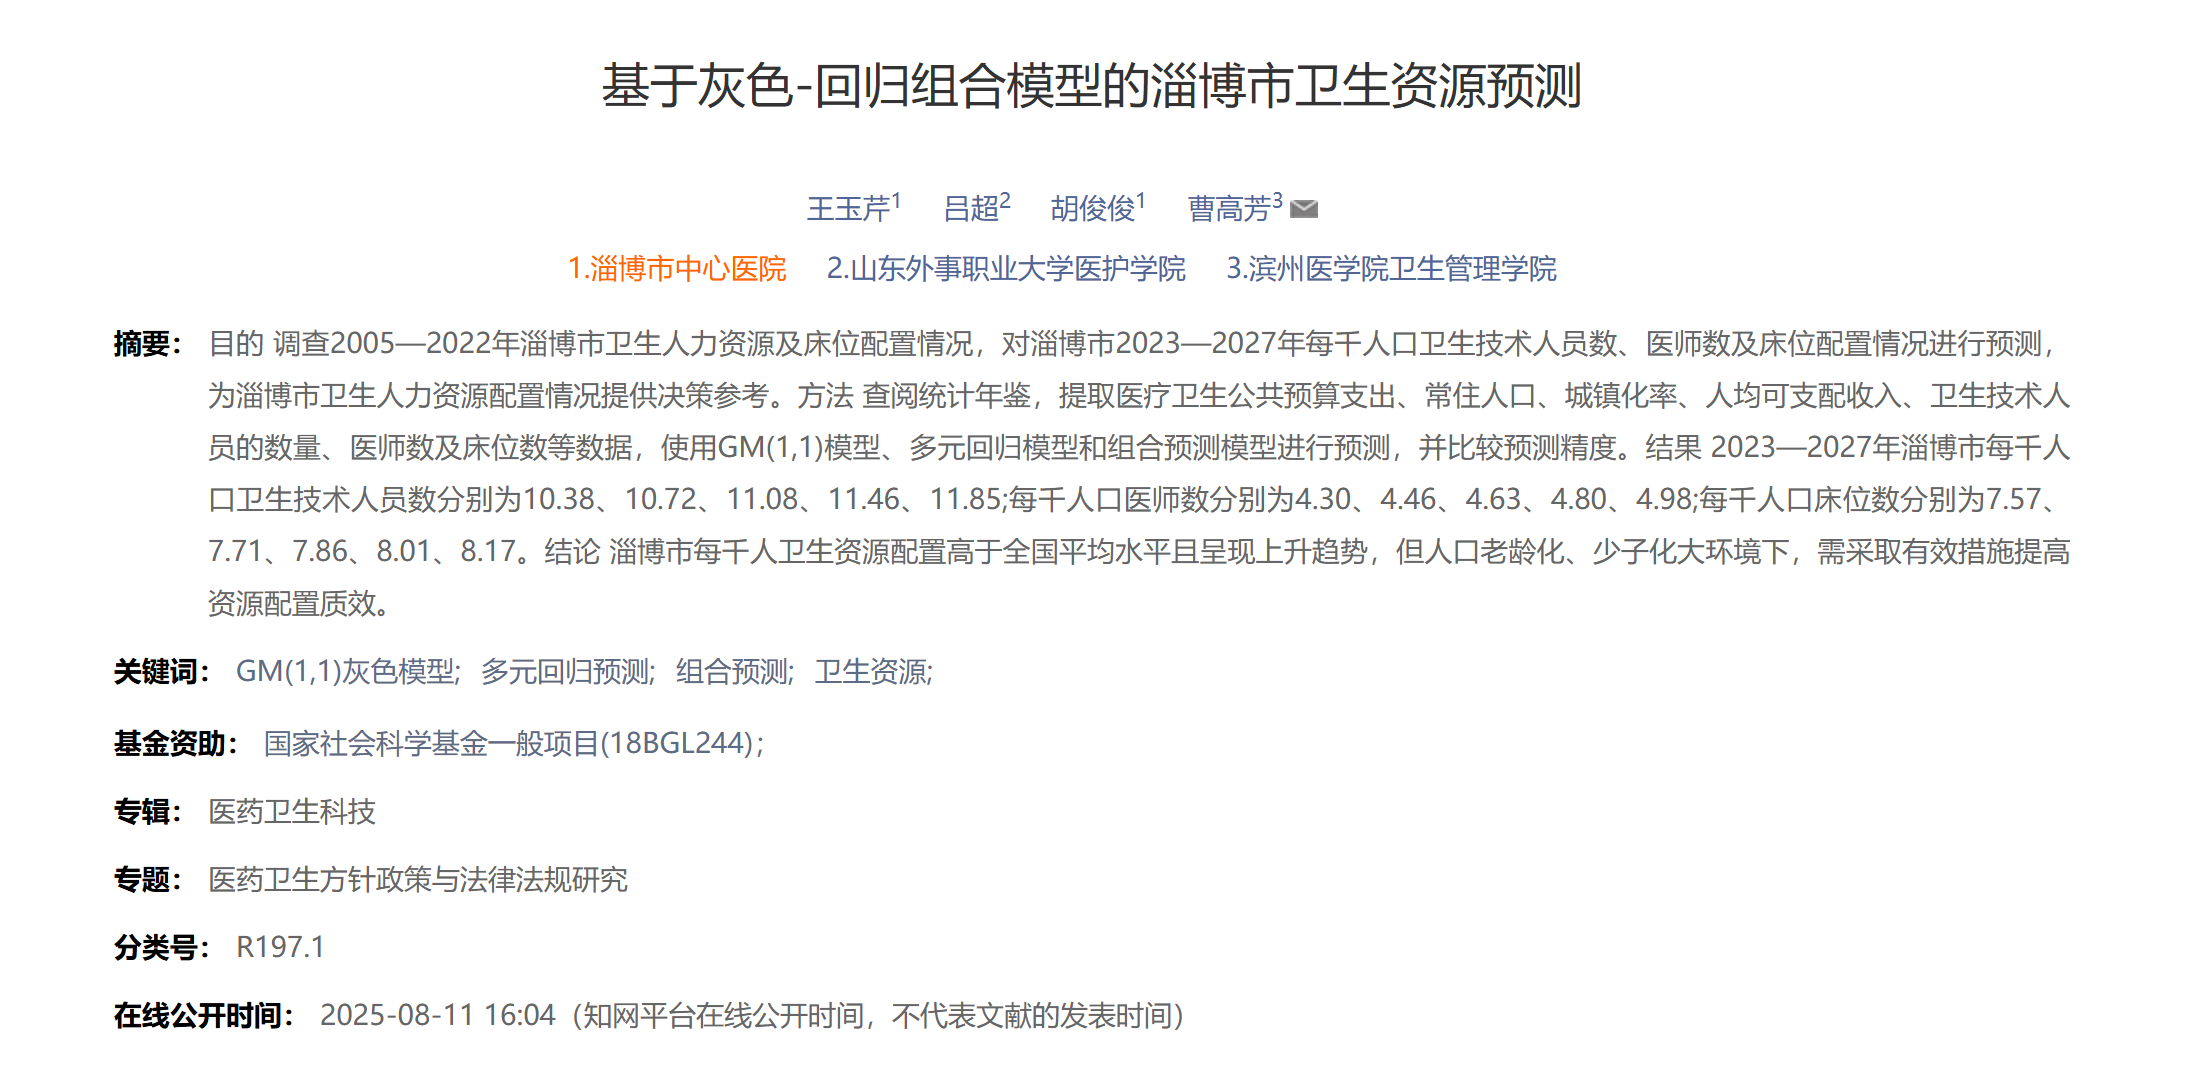
\includegraphics[width=0.8\textwidth]{essay2.png}
            \end{column}
        \end{columns}
    \end{frame}

    \section{论文研究}

    \begin{frame}{背景分析} 
        
    \end{frame}
    \section{Future Job Growth}

    \begin{frame}
        \frametitle{Future Job Growth}
        \begin{columns}
            \begin{column}{0.5\textwidth}
                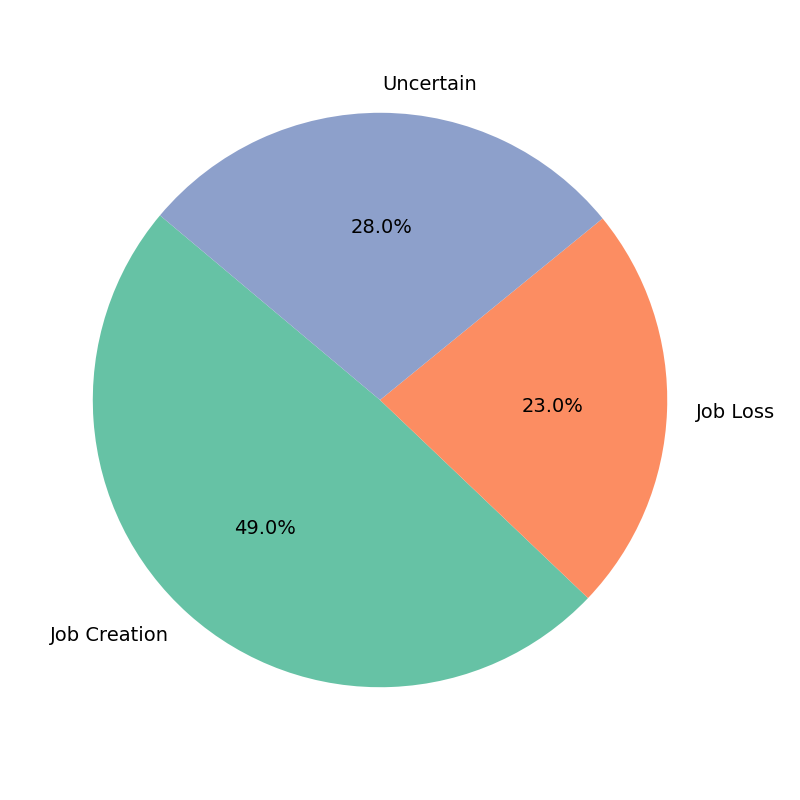
\includegraphics[width=0.85\textwidth]{ai_impact_on_jobs_pie.png}
                
                More companies expect jobs growth.
            \end{column}
            \begin{column}{0.5\textwidth}
                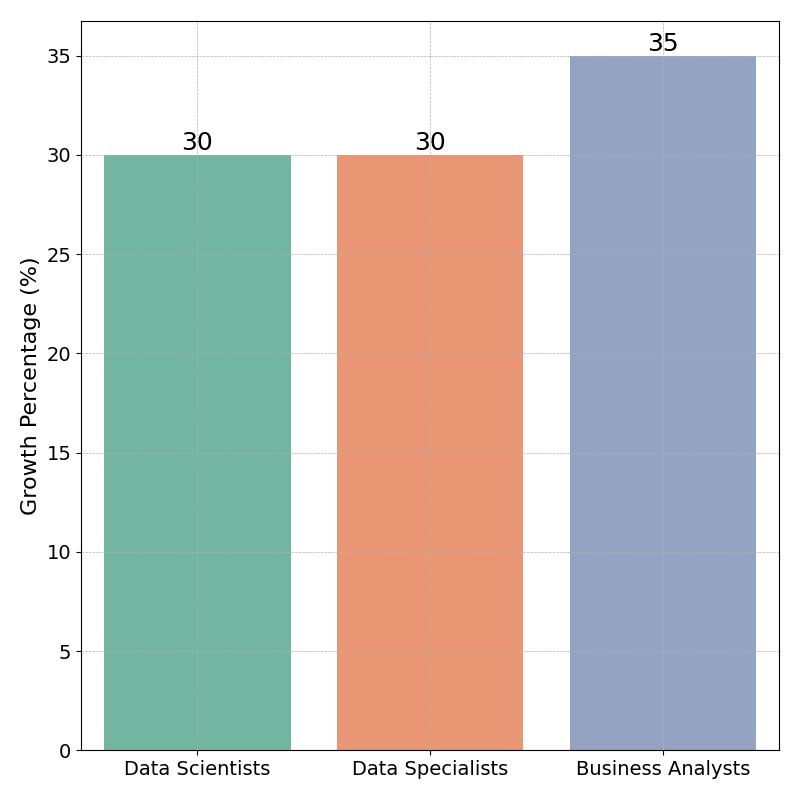
\includegraphics[width=0.85\textwidth]{ai_linked_roles_growth.png}
                AI-linked roles are expected to swell
            \end{column}
        \end{columns}
    \end{frame}

    \section{The End}

    \begin{frame}
        \frametitle{Conclusion}
            \begin{quote}
                \textbf{ AI will not replace us but \textcolor{structure}{\large reshape how
                        we work}. It is a catalyst for progress, pushing us toward more creative,
                        meaningful, and higher-value work.}        
                        \newline
                        \begin{center}
                        \textbf{\textcolor{structure}{\Large Let us embrace its potential to enhance our lives and career!}}
                \end{center}
            \end{quote}   
    \end{frame}

    \begin{frame}
        \frametitle{References}
        \begin{thebibliography}{}

            \bibitem{技术革命与就业率}
            Mark, C. Bank of England.(2018, September 14). "The Future of Work".
            Retrieved from \url{https://www.bankofengland.co.uk/-/media/boe/files/speech/2018/the-future-of-work-speech-by-mark-carney-slides.pdf}
            
            \bibitem{AI同理心}
            Bethany, C.\& Jessica, C. (2023, September 5). Opinion: Here are the jobs AI will impact most. 
            Retrieved from \url{https://www.cnn.com/2023/09/05/opinions/artificial-intelligence-jobs-labor-market/index.html}
            
            \bibitem{AI不一定更好}
            Catherine, T.(2023, July 22). ‘It almost doubled our workload’: A
            I is supposed to make jobs easier. These workers disagree. 
            Retrieved from \url{https://www.cnn.com/2023/07/22/tech/ai-jobs-efficiency-productivity/index.html}
            
            \bibitem{AI不一定更好} 
            Catherine, T.(2023, January 26). Plagued with errors: 
            A news outlet’s decision to write stories with AI backfires. 
            Retrieved from \url{https://www.cnn.com/2023/01/25/tech/cnet-ai-tool-news-stories/index.html}
            \end{thebibliography}
    \end{frame}
    \begin{frame}
        \frametitle{References}
    \begin{thebibliography}{}   
        \bibitem{AI新增就业}
        Ian, S. \& Kate, W.(2023, May). These are the jobs most likely to be lost – and created – because of AI \url{https://www.weforum.org/stories/2023/05/jobs-lost-created-ai-gpt/}
        
        \end{thebibliography}
    \end{frame}
            
    %\bibliographpage

    \QApage

\end{document}
